\chapter{MultiVeStA: Statistical Model Checking of PMaude Specifications}

As mentioned before, MultiVeStA is an extension of both VeStA and PVeStA that can be used to perform statistical model checking of PMaude specifications. Hence, the main purpose of this chapter is to present a general introduction to understand how MultiVeStA works, and how it can be used to verify PMaude specifications, obtained with the encoding from the previous chapter.

\section{MultiVeSta's components and processes}
First and foremost, the MultiVeSta tool was developed by Andrea Vandin, and it is available to download in a public repository in GitHub \cite{multiGit}. The main components of the tool are:
\begin{itemize}
    \item \textbf{Maude-3.0+yices2:} A folder that contains the Maude distribution.
    \item \textbf{apmaude.maude:} A Maude file that contains the necessary sorts, equations and rules to extend any PMaude specification, so it can be checked using the tool. 
    \item \textbf{multivesta.jar:} A java executable that runs the simulations using the specified PMaude model, the MultiQuaTEx query, and the simulation parameters.
\end{itemize}

To run simulations of a specific PMaude specification, it is necessary to pass to the tool:

\begin{itemize}
    \item \textbf{model.maude:} A Maude file, that contains the specification of the PMaude model that is going to be verified.
    \item \textbf{query.multiquatex:} A MultiQuaTEx file, with the quantitative temporal logic formula written in the MultiQuaTEx language, that will be used to verify the model.
    \item \textbf{Simulations Parameters:} There are multiple parameters to take into account when performing simulations with the tool:
    \begin{itemize}
        \item $\alpha$ and $\delta$, already explained in section 2.7.
        \item $bs$, which defines the number of simulations that each batch will contain (this parameter will be further detailed in the current section).
    \end{itemize}
\end{itemize}
With these components, it is then possible to run the simulations and obtain the results of the query, as seen in Figure \ref{fig:multi1}.
\begin{figure}[h]
    \centering
    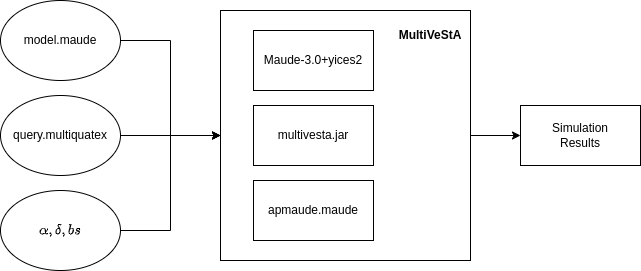
\includegraphics[scale = 0.5]{images/multi1.png}
    \caption{MultiVeSta's components}
    \label{fig:multi1}
\end{figure}
The way MultiVeStA obtains these simulation results, can be defined in the following steps:
\begin{enumerate}
    \item MultiVeStA performs $bs$ number of simulations and calculates the confidence interval based on the results obtained in each one of the simulations. Each simulation consists of:
        \begin{enumerate}
            \item Get the initial state of the system $s_0$ by running \textit{model.maude}, which includes the theory specified in \textit{apmaude.maude}, using the \textit{Maude-3.0+yices2} distribution.
            \item Evaluate the MultiQuaTEx formula in \textit{query.multiquatex} over $s_0$. If the formula is satisfied, then the simulation ends and the result of the query is returned. Otherwise, MultiVeStA performs one step in the simulation, to get the next state $s_i$.
            \item Repeat step b with the new state $s_i$, until reaching a state where the formula is satisfied and the results are returned. 
        \end{enumerate}
    As shown in section 2.7, the result of a MultiQuaTEx formula is a floating point value. Therefore, with each one of the values returned by the query in each simulation, the confidence interval of the batch is calculated.
    
    \item If the confidence interval satisfies the parameter $\alpha$ and $\delta$ i.e. the real value of the query $x$ has a probability $(1-\alpha)*100\%$ of being in the interval $[\bar{x} - \frac{\delta}{2},\bar{x} + \frac{\delta}{2}]$, where $\bar{x}$ is the current value calculated for the query using the simulations, then MultiVeStA returns the results and ends it execution. If not, then MultiVeStA will send another batch of simulations until the confidence interval is finally reached.
\end{enumerate}
In general, the complete process can be viewed in the following flowchart:
\begin{figure}[H]
    \centering
    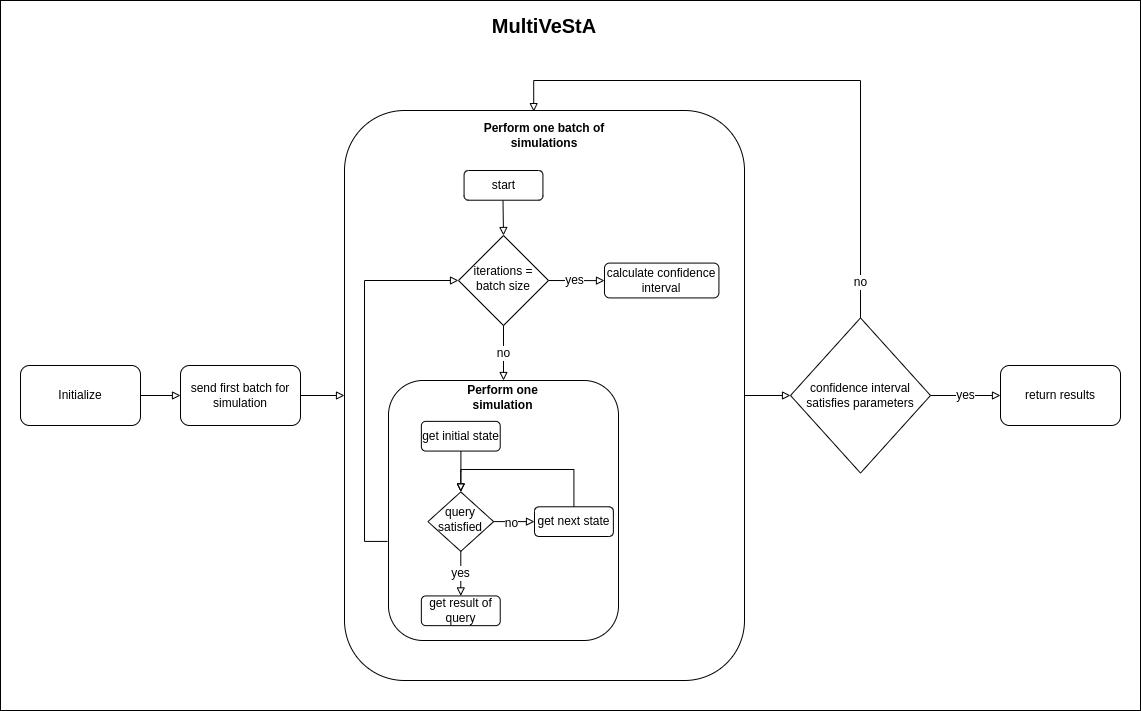
\includegraphics[scale = 0.4]{images/multi3.png}
    \caption{Flowchart of MultiVeStA's process}
    \label{fig:multi3}
\end{figure}

Having understood how the general process to perform simulations in MultiVeStA is done, it is necessary to define how to modify a PMaude specification to be able to run it with the tool. To do this, in the next section a general explanation will be given that illustrates how individual simulations work (sub-steps a, b and c from the step 1), and how this can be achieved by including new elements into the PMaude models that are going to be verified.

\section{MultiVeStA and Maude interaction}
The way MultiVeStA sends and retrieves information from Maude, is through the Maude console. Initially, MultiVeStA loads the apmaude.maude and model.maude file through the Maude console. Then, MultiVeStA sends commands to the Maude console and Maude executes these commads. Finally, MultiVeStA reads these results from the Maude's console and use them to calculate the results of the simulations. This process is captured in the following sequence diagram:

\begin{figure}[H]
    \centering
    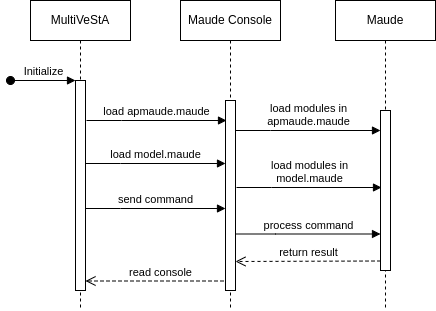
\includegraphics[scale = 0.6]{images/multi4.png}
    \caption{Sequence diagram of MultiVeStA and Maude interaction}
    \label{fig:multi4}
\end{figure}

In order to fully detail the process specified in Figure \ref{fig:multi4}, it is necessary to define some preliminary operators and equations contained in apmaude.maude and model.maude. Hence, the following list contains the description of these structures and their respective definitions:
\begin{itemize}
    \item \textbf{Scheduler:} the scheduler is a structure that contains the current number of steps or transitions in the simulation, represented as a float number, and a list of scheduler elements. In Maude it is specified as:
    \begin{maude}

op {_|_} : Float ScheduleList -> Scheduler . \end{maude}
    Each one of the scheduler elements corresponds to a pair that contains a message that identifies the next rewriting rule to be applied, and a float number that specifies in which step of the simulation the rule is going to be applied. They also contain a third value, which is a natural number that is used as a flag to drop or keep scheduler elements when inserted (this will be explained in more detail in the \texttt{insert} equation). In Maude it is defined as:
    \begin{maude}
    
op [_,_,_] : Float Msg Nat -> ScheduleElem [ ctor ] .
op [_,_] : Float Msg -> ScheduleElem .

var t1 : Float .
var M1 : Msg .

eq [ t1 , M1 ] = [ t1 , M1 , 0] . \end{maude}
    The scheduler forms part of the system states. Thus, to be able to include it in the configuration, the sort \texttt{Scheduler} is a subsort of the sort \texttt{Configuration}.
    \begin{maude}
    
subsort Scheduler < Configuration . \end{maude}
    
    The scheduler is a very important part of the simulation process, since it will be in charged of determining the next transition or rewriting rule to be applied to the model's current configuration during a simulation. Associated to the scheduler, there is an operator named \texttt{insert}, that allows to insert new elements in the scheduler list. It is defined as:
    \begin{maude}
    
op insert : Scheduler ScheduleElem -> Scheduler .
op insert : ScheduleList ScheduleElem -> ScheduleList .  

vars t1 t2 gt : Float .
var SL : ScheduleList .
var e : ScheduleElem .
vars M1 M2 : Msg .
var p : Nat .

eq insert({ gt | SL },e) = { gt | insert(SL,e) } .
eq insert(SL , [ t2 , M2 , 1]) = SL .
eq insert( nilSL , [ t2 , M2 , 0]) = [ t2 , M2 , 0] .
eq insert([ t1 , M1 , p] ; SL , [ t2 , M2 , 0]) = 
   if t1 < t2 
    then [ t1 , M1 , p] ; insert(SL, [ t2 , M2 , 0]) 
    else ([ t2 , M2 , 0] ; [ t1 , M1 , p] ; SL) 
   fi . \end{maude}
    What this equation does is to take a scheduler, a scheduler element, and insert the element inside the list of the scheduler according to the float number in the scheduler elements, like a priority queue. In the end, the first element in the list is going to contain the message that specifies the next rule to be executed, since it has the smallest step. If the value of the flag is 1, then the element is not inserted, but if it is 0, then the element is inserted.  
        
    Moreover, the scheduler induces an implicit constraint over the model specified in model.maude: the selection of the next rule to be applied must be deterministic, in the sense that in every state of the simulation the next rule must be pre-selected, instead of the non-deterministic mechanism for choosing rules in Maude. For this reason, model.maude must have a rule or equation that chooses the next rule during the simulations. 

    \item \textbf{Random Counter:} the random counter is a structure that contains a natural number, that will be used to select random numbers, similar to the \texttt{COUNTER} module explained in section 2.6. The reason for not using the \texttt{COUNTER} module in MultiVeStA and using a structure that saves the value of the counter, is because during simulation MultiVeStA resets the Maude console. Therefore, if the \texttt{COUNTER} module is used, the value of the counter to select random numbers will always be 0. With every application of a rule, the idea is to change the number of the random counter, so the generated random numbers are different in every simulation step. In Maude, the random counter is defined as:
    \begin{maude}

op randomCounter : Nat -> Object [ ctor ] . \end{maude}
    The random counter has sort \texttt{Object} since it is also part of the system states.

    \item \textbf{States of the Simulation:} as defined in section 2.4, states of a Maude specification are represented with a term. In this case, the states in the simulations have sort \texttt{Configuration} and are defined as:
    \begin{maude}

var gt : Float .
var SL : ScheduleList .
var C : Configuration .
var n : Nat .

{gt | SL} {C randomCounter(n)} \end{maude}
    where \texttt{\{gt | SL\}} is a term of sort \texttt{Scheduler} and \texttt{C} is a term of sort \texttt{Configuration}. The curly brackets \texttt{\{\_\}} are an operator defined as: 
    \begin{maude}
    
op { _ } : Configuration -> Configuration [ ctor ] . \end{maude}
    \texttt{C} represents the original states of the model without the required elements to run it with MultiVeStA, i.e the scheduler and the random counter. For instance, in the clock example from section 2.7, the term: 
    \begin{maude}
    
< myClock : Clock | time: Nat, battery: Float, state: State > \end{maude}
    represents the configuration \texttt{C}. Finally, \texttt{randomCounter(n)}, as explained before, is an object that contains a natural number that will be used to generate random numbers. Additionally, there is an operator named \texttt{tick}, defined as:
    \begin{maude}

op tick : Configuration -> Configuration .
op mytick : Scheduler -> Configuration .

vars t1 gt : Float .
var C : Configuration .
var sc : Scheduler .
var p : Nat .
var SL : ScheduleList .
var M1 : Msg .

eq tick( sc C ) = mytick(sc) C .
eq mytick({ gt | [ t1 , M1 , p] ; SL }) = M1 { t1 | SL } .
eq mytick({ gt | nilSL }) = { gt | nilSL } . \end{maude}
    its main purpose is to take out the first element from the scheduler list, add the message inside the scheduler element (i.e. \texttt{M1}) to the current state of the simulation, and replace \texttt{gt} with the step inside the scheduler element (i.e. \texttt{t1}).  
 
    \item\textbf{Initial State:} as the name suggests it, this term corresponds to the initial state of the system. It is defined as:
    \begin{maude}

op init : -> Configuration .
op initState : -> Configuration .
eq initState = closeWorldExceptScheduler(init) [ owise ] \end{maude}
    For the initial state there are two operators involved: \texttt{init} and \texttt{initState}. \texttt{init} is a constant of sort \texttt{Configuration}, that will have to be defined by the user in the model.maude file with the equation:
    \begin{maude}

eq init = {0.0 | nilSL} C0 randomCounter(0). \end{maude}
    It initializes the scheduler with steps equal to 0.0 and an empty list of scheduler elements written as \texttt{nilSL}. The term \texttt{C0} is the configuration that represents the initial state of the model, and \texttt{randomCounter} starts with the value 0. \texttt{initState} corresponds to the application of the equation \texttt{closeWorldExceptScheduler} over the constant \texttt{init}. This equation is defined as:
    \begin{maude}
    
op closeWorldExceptScheduler : Configuration -> Configuration .
eq closeWorldExceptScheduler(sc C) = sc { C } .\end{maude}
    The equation is used to group all the objects from the configuration and isolate the scheduler. Thus, inside the curly brackets the objects will be the system state and the random counter: \texttt{\{C randomCounter(n)\}}.   
    
\item \textbf{Scheduler Rule:} Continuing with the observation made about the scheduler, a rule $SR$ will be defined inside model.maude, that is in charge of selecting the next rule that is going to be applied to the current system state. For that reason, the $SR$ rule must insert in the scheduler list the scheduler element that has the message that represents the rule chosen by the $SR$ rule.

\item \textbf{Rule Associated to a Message:} Each one of the scheduler elements contains a message \texttt{Mi} that is going to be used to identify the next rule that is going to be executed. Therefore, the associated rule must consider in its definition the presence of the message \texttt{Mi}. Based on this, the rule $R_{M_i}$ can be defined as the rule associated with the message \texttt{Mi}, and specified as:
\begin{maude}

rl : Mi {gt | SL} {C randomCounter(n)} =>
        {gt | SL} {C' randomCounter(n)} .\end{maude}
The rule eliminates the message from the configuration and changes the term \texttt{C} to \texttt{C'}, indicating that the rule has been applied, and the state of the system has been changed.

\item \textbf{Val operator:} This operator is used to define observations over the states of the system, allowing to extract valuable information that can be then evaluated in the MultiQuaTEx query using the \texttt{s.rval()} function, explained in section 2.7. It is defined as:
\begin{maude}

op val : Nat Configuration -> Float .
op val : String Configuration -> Float . \end{maude}
Where the natural number and the string serve as identifiers, and the configuration represents the state where the observation is going to be made. For example, recall the state observation \texttt{s.rval("isBrk")} in the clock example from section 2.7. For MultiVeStA to be able to get the value for \texttt{s.rval("isBrk")} when evaluating the MultiQuaTEx query, the user must define in model.maude the corresponding equation with the \texttt{val} operator and the same identifier, in this case \texttt{"isBrk"}. The resulting equation in the model.maude files is:
\begin{maude}

var C : Configuration .
var gt : Float .
var SL : ScheduleList .
var cl : Oid .
var n : Nat .

--- returns 1.0 if the clock is broken, 0.0 if not
op isBroken : Configuration -> Float .
eq isBroken(< cl : Clock | state: broken, attrSet > C) = 1.0 .
eq isBroken(< cl : Clock | state: working, attrSet > C) = 0.0 .

--- Eval if the clock is broken
eq val("isBrk", {gt | SL} {C randomCounter(n)}) = isBroken(C) .\end{maude}

It is also important to mention, that ther are two predefined state observations in MultiVeStA, which are \texttt{s.rval("steps")} and \texttt{s.rval("time")}. The former returns the number of ticks done in the simulation, and the latter returns the value \texttt{gt} of the scheduler \texttt{\{gt | SL\}}.
\end{itemize}

Having defined the preliminary structures used in the simulations, the complete process of a single simulation will be described in detail as a series of steps:
\begin{enumerate}
    \setcounter{enumi}{-1}
    \item The user defines the initial state as:
    \begin{maude}
    
eq init = {0.0 | nilSL} C0 randomCounter(0) . \end{maude}
    and the state observations:
    \begin{maude}
    
eq val("obs1", {gt | SL} {C randomCounter(n)}) = ...
eq val("obs2", {gt | SL} {C randomCounter(n)}) = ...
...
eq val("obsn", {gt | SL} {C randomCounter(n)}) = ...\end{maude}
    inside model.maude.
    \item MultiVeStA loads the apmaude.maude and the model.maude files to Maude, using the Maude console.
    \item MultiVeStA sends the command \texttt{rew initState}. 
    \begin{enumerate}
        \item Maude reduces the \texttt{initState} term:
        \begin{maude}

initState $\rightarrow$ {0.0 | nilSL} {C0  randomCounter(0)} .\end{maude}
        \item The rule $SR$ chooses the next rule to be executed, represented with the message \texttt{Mi}, by inserting an element in the scheduler list. The random counter is also incremented:
        \begin{maude}

{0.0 | nilSL }        $\xrightarrow{SR}$   insert({0.0 | nilSL },[ gt + 1.0 , Mi])
{C0 randomCounter(0)}       {C0 randomCounter(0+1)}\end{maude}
        \item Maude reduces the terms:
        \begin{maude}
        
insert({0.0 | nilSL },[ 0.0 + 1.0 , Mi]) $\rightarrow$ {0.0 | [1.0 , Mi] } 
{C0 randomCounter(0+1)}                     {C0 randomCounter(1)}\end{maude}
    \end{enumerate}

\item MultiVeStA reads the Maude console and saves the current configuration. The saved configuration will be defined as \texttt{Conf}.

\item MultiVeStA evaluates the query in query.multiquatex, using the user defined equations for the \texttt{val} operators, to calculate the \texttt{s.rval()} state observations. To do this, for every \texttt{s.rval("obs")} in the query, MultiVeStA sends to Maude the command \texttt{red val("obs", Conf)}, and obtains the float number returned by the equation. Using these results of the \texttt{val} equations, then MultiVeStA is able to evaluate the query.

\item If the query is satisfied, then MultiVeStA gets the float number returned by the query. If not, then continue with step 6.

\item MultiVeStA sends the command \texttt{rew tick(Conf)}.
    \begin{enumerate}
        \item Maude reduces the term \texttt{rew tick(Conf)}:
        \begin{maude}

tick({gt | [gt' , Mi]}     $\rightarrow$  Mi {gt' | nilSL }
     {C randomCounter(n)})    {C randomCounter(n)}\end{maude}
        \item Maude rewrites the term with the rule associated with the message \texttt{Mi}:
        \begin{maude}
        
Mi {gt' | nilSL}    $\xrightarrow{R_{M_i}}$ {gt' | nilSL }
{C randomCounter(n)}     {C'  randomCounter(n)}\end{maude}
        In this case, the term \texttt{C'} represents the next state of the model after applying $R_{M_i}$ over \texttt{C}.
        \item The rule $SR$ chooses the next rule to be executed, represented with the message \texttt{Mj}:
        \begin{maude}

{gt' | nilSL }        $\xrightarrow{SR}$   insert({gt' | nilSL},[gt' + 1.0 , Mj])
{C' randomCounter(n)}       {C' randomCounter(n+1)}\end{maude}
        
        \item Maude reduces the terms:
        \begin{maude}
        
insert({gt' | nilSL},[gt' + 1.0 , Mj]) $\rightarrow$ {gt' | [gt' + 1.0 , Mj]} 
{C' randomCounter(n+1)}                   {C' randomCounter(n+1)}\end{maude}
    \end{enumerate}

    \item Repeat step 3 and 4.
    
    \item If the query is satisfied, then get the float number returned by the query. If not, then repeat steps 6 trough 8 over the previous configuration \texttt{Conf}, until the formula is satisfied.
\end{enumerate}
The complete process can be visualized in a sequence diagram, that extends the previous one presented in figure \ref{fig:multi4}:

\begin{figure}[H]
    \centering
    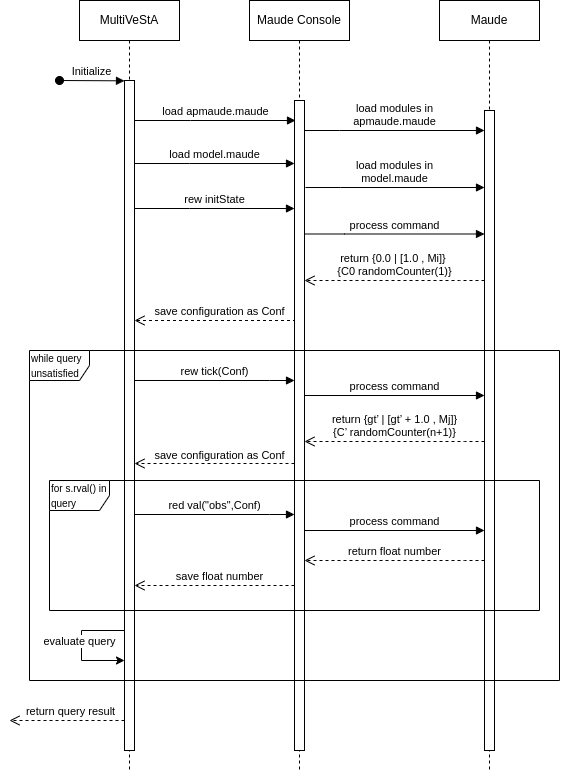
\includegraphics[scale = 0.5]{images/multi5.png}
    \caption{Extension of sequence diagram in Figure \ref{fig:multi4}}
    \label{fig:multi5}
\end{figure}

Based on this introduction to MultiVeStA and chapter 3, the next section will present the integration between the rewriting logic approach to probabilistic Event-B and MultiVeStA.

\section{Using MultiVeStA to verify $\mathscr{R}_\mathscr{M}$}

To verify properties of probabilistic Event-B models encoded as probabilistic rewrite theories $\mathscr{R}_\mathscr{M}$, it is necessary to list the required components to complete this process. First, the mandatory theory to specify the encoded model that wants to be checked, should be included, i.e. the rewrite theory $\mathscr{R}$ with the modules \texttt{SAMPLER}, \texttt{EB-CORE}, \texttt{EBCONTEXT} and \texttt{EBMACHINE}. Then, the model.maude file should specify the system module \texttt{MODEL}, which includes $\mathscr{R}$. The interaction between the model and MultiVeStA is specified in Figure \ref{fig:multi6}.       
\begin{figure}[H]
    \centering
    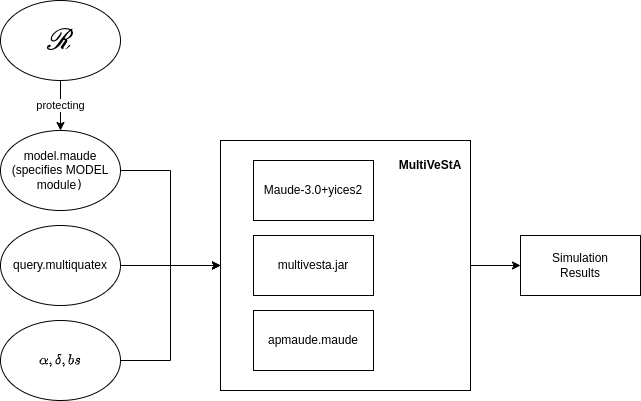
\includegraphics[scale = 0.5]{images/multi6.png}
    \caption{Interaction between the encoded model and MultiVeStA}
    \label{fig:multi6}
\end{figure}
Even though the simulation process is the same, as described in Figures \ref{fig:multi3} and \ref{fig:multi5}, it is important to consider and identify the differences that arise when the simulation of the encoded models is done. Hence, the rest of this section will specify and describe how the same series of steps explained in section 4.2, function with the specific case of probabilistic rewrite theories $\mathscr{R}_\mathscr{M}$. Initially, the following list contains the required definitions to understand the simulation process:
\begin{itemize}
    \item \textbf{States of the Simulation in $\mathscr{R}_\mathscr{M}$:} Given that the general definition for a state of a model that is going to be verified with MultiVeStA is:
    \begin{maude}

{gt | SL} {C randomCounter(n)}\end{maude}
    Then, replacing the term \texttt{C} with the term that represents states in $\mathscr{R}_\mathscr{M}$, the resulting configuration is:
    \begin{maude}
    
{gt | SL} {$\mathfrak{C} \ \mathfrak{M}_{i}  \ \mathfrak{E}$ randomCounter(n)}\end{maude}
    
    \item \textbf{Initial State in $\mathscr{R}_\mathscr{M}$:} the initial state of the simulation is specified with the operator \texttt{init} and it is defined as:
    \begin{maude}

eq init = {0.0 | nilSL} $\mathfrak{C} \ \mathfrak{M}_{0}  \ \mathfrak{E}$ randomCounter(0) .\end{maude}
    
    \item \textbf{Messages in $\mathscr{R}_\mathscr{M}$:} The messages that identify the next rule to be applied, are defined for the translated models $\mathscr{R}_\mathscr{M}$ with the operator:
    \begin{maude}

op _<-_ : Oid Content -> Msg .\end{maude}
    
    where the \texttt{Oid} is the object identifier of the machine $\mathfrak{M}$, and the second parameter of sort \texttt{Content} is used to identify the rule that is going to be applied. For example for the brake system example explained in section 2.3 and chapter 3, the message that identifies the push pedal rule in the model would be:
    \begin{maude}

op RulePushPedal : -> Content [ ctor ] .
'BrakeSystem <- RulePushPedal\end{maude}

    \item \textbf{Scheduler Rule in $\mathscr{R}_\mathscr{M}$:} In the case of translated models $\mathscr{R}_\mathscr{M}$ by the encoding, the $SR$ rule explained in the previous section corresponds to the $chooseEvt$ rule. To integrate the $chooseEvt$ rule with the scheduler, an auxiliary equation is used to identify the selected rule and insert it to the scheduler. The definition of this rule is:
    \begin{maude}

var gt : Float .
var n : Nat .
var SL : ScheduleList .
var MNAME : Oid .
var ruleQid : Qid .
 
op scheduleEvent : Configuration -> Configuration .
eq scheduleEvent( { gt | SL } 
                  {$\mathfrak{C} \ \mathfrak{M}_{i} $ 
                  < events  : Events  | state: ( ev(ruleQid, execute) ) > 
                  randomCounter(n)} )
                 =
                  insert({ gt | SL },
                         [ gt + 1.0 , (MNAME <- qidToContent(ruleQid)),0]) 
                  {$\mathfrak{C} \ \mathfrak{M}_{i} $ 
                  < events  : Events  | state: ( ev(ruleQid, execute) ) > 
                  randomCounter(n)} .\end{maude}
    where \texttt{MNAME} is object identifier of the machine $\mathfrak{M}_{i}$, \texttt{ruleQid} is the quoted identifier of the selected rule, and \texttt{qidToContent} is an equation that maps the \texttt{Qid} of every rule, to a term of sort \texttt{Content}.

    \item \textbf{Rule $R_{M_i}$ in $\mathscr{R}_\mathscr{M}$}: the $execEvt_{e_i}$ rule in $\mathscr{R}_\mathscr{M}$, corresponds to the $R_{M_i}$ rule. To adapt each one of the rules $execEvt_{e_i}$ to resemble the behavior of $R_{M_i}$, it is necessary to include in the definition of $execEvt_{e_i}$, the message that represents the event. For example, if the rule $execEvt_{e_i}$ is defined as:
    \begin{maude}

rl [eventEi]: { gt | SL } $\mathfrak{C} \ \mathfrak{M}_{i}  \ \mathfrak{E}$ randomCounter(n)
              => 
              { gt | SL } $\mathfrak{C} \ \mathfrak{M}_{j}  \ \mathfrak{E}$ randomCounter(n)\end{maude}
    then, the adapted rule is:
    \begin{maude}

rl [eventEi]: (MNAME <- eventEi) { gt | SL } $\mathfrak{C} \ \mathfrak{M}_{i}  \ \mathfrak{E}$ randomCounter(n)
              => 
              { gt | SL } $\mathfrak{C} \ \mathfrak{M}_{j}  \ \mathfrak{E}$ randomCounter(n)\end{maude}
where \texttt{MNAME} is the \texttt{Oid} of the machine, and \texttt{eventEi} is a term of sort content that identifies the rule.
\end{itemize}

With these definitions, it is now possible to redefine the simulation steps explained in the previous section:

%---------------------------------------------------------------------------------------------
%---------------------------------------------------------------------------------------------
%---------------------------------------------------------------------------------------------
%---------------------------------------------------------------------------------------------
%---------------------------------------------------------------------------------------------


\begin{enumerate}
    \setcounter{enumi}{-1}
    \item The user defines the initial state as:
    \begin{maude}
    
eq init = {0.0 | nilSL} $\mathfrak{C} \ \mathfrak{M}_{0}  \ \mathfrak{E}$ randomCounter(0) . \end{maude}
    and the state observations:
    \begin{maude}
    
eq val("obs1", {gt | SL} {$\mathfrak{C} \ \mathfrak{M}  \ \mathfrak{E}$ randomCounter(n)}) = ...
eq val("obs2", {gt | SL} {$\mathfrak{C} \ \mathfrak{M}  \ \mathfrak{E}$ randomCounter(n)}) = ...
...
eq val("obsn", {gt | SL} {$\mathfrak{C} \ \mathfrak{M}  \ \mathfrak{E}$ randomCounter(n)}) = ...\end{maude}
    inside model.maude.
    
    \item MultiVeStA loads the apmaude.maude, the files that contain the modules \texttt{SAMPLER}, \texttt{EB-CORE}, \texttt{EBCONTEXT} and \texttt{EBMACHINE}, and the model.maude file which includes the previous modules.
    \item MultiVeStA sends the command \texttt{rew initState}. 
    \begin{enumerate}
        \item Maude reduces the \texttt{initState} term:
        \begin{maude}

initState $\rightarrow$ {0.0 | nilSL} {$\mathfrak{C} \ \mathfrak{M}_{0}  \ \mathfrak{E}$  randomCounter(0)} .\end{maude}
        \item The rule $chooseEvt$ chooses the next rule to be executed. The random counter is also incremented:
        \begin{maude}
 
{0.0 | nilSL }             $\xrightarrow{chooseEvt}$      scheduleEvent({0.0 | nilSL } 
{$\mathfrak{C} \ \mathfrak{M}_{0} \ \mathfrak{E}$ randomCounter(0)}              {$\mathfrak{C} \ \mathfrak{M}_{0} \ \mathfrak{E'}$ randomCounter(0+1)})\end{maude}
        where $\mathfrak{E'} = \texttt{<events:Events|state:(ev(ruleQid,execute))}$  
        
        \item Maude reduces the terms:
        \begin{maude}
                                
scheduleEvent({0.0 | nilSL } $\rightarrow$ insert({0.0 | nilSL },[0.0+1.0,$MG$,0])
{$\mathfrak{C} \ \mathfrak{M}_{0} \ \mathfrak{E'}$ randomCounter(0+1)})   {$\mathfrak{C} \ \mathfrak{M}_{0} \ \mathfrak{E'}$ randomCounter(1)}\end{maude}

        \begin{maude}
                                    
insert({0.0 | nilSL },[0.0+1.0,$MG$,0]) $   \rightarrow$ {0.0 | [1.0 , $MG$] }
{$\mathfrak{C} \ \mathfrak{M}_{0} \ \mathfrak{E'}$ randomCounter(1)}                {$\mathfrak{C} \ \mathfrak{M}_{0} \ \mathfrak{E'}$ randomCounter(1)}\end{maude}

Where $MG = \texttt{(MNAME<-qidToContent(ruleQid))}$
    \end{enumerate}

\item Do steps 3, 4 and 5 from the previous section.

\item MultiVeStA sends the command \texttt{rew tick(Conf)}.
    \begin{enumerate}
        \item Maude reduces the term \texttt{rew tick(Conf)}:
        \begin{maude}

tick({gt | [gt' , $MG$]}     $\rightarrow$  $MG$ {gt' | nilSL }
{$\mathfrak{C} \ \mathfrak{M}_{i} \ \mathfrak{E'}$ randomCounter(n)})     {$\mathfrak{C} \ \mathfrak{M}_{i} \ \mathfrak{E'}$ randomCounter(n)}\end{maude}
        \item Maude rewrites the term with the rule associated with the message \texttt{Mi}:
        \begin{maude}
        
$MG$ {gt' | nilSL }    $\xrightarrow{execEvt_{e_i}}$ {gt' | nilSL }
{$\mathfrak{C} \ \mathfrak{M}_{i} \ \mathfrak{E'}$ randomCounter(n)}     {$\mathfrak{C} \ \mathfrak{M}_{j} \ \mathfrak{E}$  randomCounter(n)}\end{maude}
        
        Where $\mathfrak{M}_{j}$ is the next system state after applying the rule $execEvt_{e_i}$. Note that $\mathfrak{E} = \langle events : Events \ | \ state: ev(e_1,unknown) ... ev(e_n, unknown) \rangle$
        \item The rule $chooseEvt$ chooses the next rule to be executed:
        \begin{maude} 

{gt' | nilSL }             $\xrightarrow{chooseEvt}$      scheduleEvent({gt' | nilSL } 
{$\mathfrak{C} \ \mathfrak{M}_{j} \ \mathfrak{E}$ randomCounter(n)}              {$\mathfrak{C} \ \mathfrak{M}_{j} \ \mathfrak{E'}$ randomCounter(n+1)})\end{maude}
where $\mathfrak{E'} = \texttt{<events:Events|state:(ev(ruleQid,execute))}$.

        \item Maude reduces the terms:
        \begin{maude}
        
scheduleEvent({gt' | nilSL }  $\rightarrow$   {gt' | [gt' + 1.0 , $MG$]}   
{$\mathfrak{C} \ \mathfrak{M}_{j} \ \mathfrak{E'}$ randomCounter(n+1)})      {$\mathfrak{C} \ \mathfrak{M}_{j} \ \mathfrak{E'}$ randomCounter(n+1)})\end{maude}
    \end{enumerate}

    \item Repeat step 3.
    
    \item If the query is satisfied, then get the float number returned by the query. If not, then repeat steps 4 trough 6 over the previous configuration \texttt{Conf}, until the formula is satisfied.
\end{enumerate}
Following this process, it is then possible to do statistical model checking over $\mathscr{R}_\mathscr{M}$ rewrite theories, and evaluate MultiQuaTEx queries. In the next section, some case studies will be presented to illustrate the interplay between the encoder and MultiVeStA.
















